\documentclass[10pt,a4paper,final]{report}
\usepackage{amsmath}
\usepackage{amsfonts}
\usepackage{listings}
\usepackage{graphicx} % Required for including images
\usepackage[font=small,labelfont=bf]{caption} % Required for specifying captions to tables and figures
\usepackage{hyperref}
\usepackage[utf8]{inputenc}
\usepackage[spanish]{babel}
\usepackage{amsthm}
\usepackage{graphicx}
\newtheorem{theorem}{Teorema}
\newtheorem{lemma}[theorem]{Lema}
\newtheorem{definition}[theorem]{Definición}
\newtheorem{proposition}[theorem]{Proposición}
\newtheorem{observation}[theorem]{Observación}
\newtheorem{corollary}[theorem]{Corolario}
\newtheorem{example}[theorem]{Ejemplo}

\newtheorem{caution}[theorem]{¡Cuidado!}



\def\powertower#1#2{#1\ifnum#2>1 ^{\powertower{#1}{\numexpr#2-1\relax}}\fi}

\def\key#1{\{#1\}}

\begin{document}



TODO: para caracterizar grupos, anillos y cuerpos, se hace algo parecido a la criba de eratóstenes.

\section{Suma y Producto: números finitos y transfinitos}


\begin{observation}
	Prima cumple Leibnitz con la suma.
\end{observation}

\begin{definition}[Suma]
	$\alpha + \beta = min \{\gamma: \gamma \neq \alpha' + \beta, \alpha + \beta' \forall \alpha'<\alpha, \beta'<\beta \}$
\end{definition}

\begin{theorem}[Los ordinales forman un grupo abeliano]
	\begin{itemize}
		\item[]
		\item $\alpha + \beta = \beta + \alpha$
		\item $\alpha + \beta = \alpha + \gamma \Leftrightarrow \beta = \gamma$
		\item $\alpha + \beta = 0 \Leftrightarrow \alpha = \beta$
		\item $\alpha + 0 = \alpha, (\alpha + \beta) + \gamma = \alpha + (\beta + \gamma), \alpha + \alpha = 0, -\alpha = \alpha$
	%	\item $\alpha0 = 0,\alpha1 = \alpha, \alpha\beta = \beta\alpha, (\alpha+\beta)\gamma= \alpha\gamma+\beta\gamma, (\alpha\beta)\gamma=\alpha(\beta\gamma)$
	\end{itemize}
\end{theorem}

\begin{proof}

%Tenemos que $\alpha + \beta = mex\{\alpha* + \beta, \alpha + \beta* \}$, donde $\alpha*$ es una variable que toma valores menores que $\alpha$ y lo análogo con $\beta$.

Llamemos $\alpha'$ a un ordinal variable que puede ser cualquier ordinal menor que $\alpha$, y si $\alpha = mex(S)$, llamemos $\alpha*$ a un ordinal que puede tomar un valor de $S$, un 'excluyente'. En ese sentido $\alpha*$ debe tomar todos los valores menores que $\alpha$ y puede tomar valores más grandes que $\alpha$. Esto es porque no cambiaría la definición de $\alpha = mex\{\alpha*\}$. Justamente $S$ puede tener huecos, como los conjuntos y las funciones de Bachmann-Howard.


\begin{itemize}

\item La conmutatividad sale directo de la definición; la asociatividad es medio aburrida de probar.


\item Veamos que $\alpha + \beta = \alpha + \gamma \Leftrightarrow \beta = \gamma$:

$\Leftarrow)$: trivial\\

$\Rightarrow)$: SPG, supongamos que $\gamma < \beta$. Entonces por la definición de suma, $\alpha + \gamma$ es un 'excluyente' en la definición de $\alpha+\beta$, es decir, pertenece a $mex\{\alpha' + \beta, \alpha + \beta' \}$ y por lo tanto es distinto a $\alpha+\beta$.

Además, $\alpha + \beta = mex\{\alpha* + \beta, \alpha + \beta* \}$. En efecto, todos los ordinales de la pinta $\alpha' + \beta, \alpha + \beta'$ son excluyentes, y cualquier otro ordinal de esa pinta que es excluyente, por lo visto recién, es distinto a $\alpha+\beta$.

\item $\alpha + 0 = mex\{\alpha* + 0, \alpha + 0*\}$. Como no hay ordinales menores que cero, tenemos que $\alpha + 0 = mex\{\alpha* + 0\}$, y por inducción transfinita se ve que esto es igual a $\alpha$.

\item $\alpha + \beta = 0 \Leftrightarrow \alpha = \beta$:

$\Leftarrow): $ Por inducción en $\alpha$. Si $\alpha=0$ es trivial. Supongamos $\alpha>0$. Entonces $\alpha + \alpha = mex\key{\alpha' + \alpha} = 0$ porque como $\alpha'+\alpha'=0$ no puede ser $\alpha'+\alpha = 0$ porque sino, por cancelación a izquierda tendríamos $\alpha = \alpha'$.

$\Rightarrow):$ Como $\alpha + \alpha = 0$ y $\alpha + \beta  = 0$, nuevamente por cancelación a izquierda tenemos que $\alpha = \beta$.

\item Es asociativa, por inducción en $\alpha + \beta$.

Si $\alpha + \beta = 0$, entonces tenemos que $\alpha = \beta$. Si $\alpha=0$ es trivial, así que supongamos $\alpha>0$.

Probemos que $(\alpha + \alpha) + \gamma = \alpha + (\alpha + \gamma)$ por inducción en $\gamma$, para todo $\alpha$. Si $\gamma = 0$ es trivial así que supongamos $\gamma > 0$.

Luego $(\alpha + \alpha) + \gamma = 0 + \gamma = \gamma$. Por otro lado, $\alpha + (\alpha + \gamma) = \key{\alpha* + (\alpha + \gamma), \alpha + (\alpha + \gamma)*} = \key{\alpha' + (\alpha + \gamma), \alpha + (\alpha' + \gamma), \alpha + (\alpha + \gamma')}$. Como $\gamma'<\gamma'$ por H.I. en $\gamma$ tenemos que $\alpha + (\alpha + \gamma') = (\alpha + \alpha) + \gamma' = \gamma'$, luego en el conjunto están todos los ordinales menores que $\gamma'$. Falta ver que no está $\gamma$ en el conjunto. La imagen mental puede ser esta, lo rojo representando elementos del conjunto:

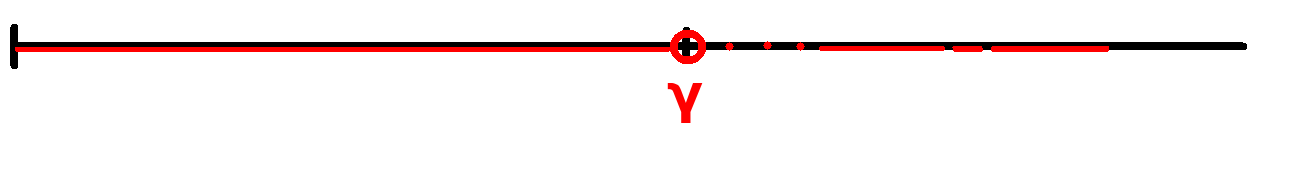
\includegraphics[scale=0.3]{mex_gamma.png}

Supongamos que $\alpha + (\alpha + \gamma') = \gamma$ para cierto $\gamma'$. Entonces sumando a izquierda a ambos lados $\alpha$ y usando que $\alpha + \alpha = 0$ obtenemos que $\alpha + \gamma' = \alpha + \gamma$, lo cuál es absurdo por la definición de la suma. Análogamente, si $\alpha' + (\alpha + \gamma) = \gamma$, sumando a ambos lados a izquierda $\gamma'$ obtenemos $\alpha + \gamma = \alpha' + \gamma$, nuevamente absurdo. Luego $\key{\alpha* + (\alpha + \gamma), \alpha + (\alpha + \gamma)*} = \key{\alpha' + (\alpha + \gamma), \alpha + (\alpha' + \gamma), \alpha + (\alpha + \gamma')} = \gamma$ como queríamos ver.

Esto prueba el caso $\alpha + \beta = 0 \forall \gamma$.

Supongamos ahora que $\alpha + \beta > 0$.

Tenemos que $(\alpha + \beta) + \gamma = mex \key{(\alpha + \beta)* + \gamma, (\alpha + \beta) +  \gamma*} = mex \key{(\alpha'+\beta) + \gamma, (\alpha + \beta') + \gamma, (\alpha + \beta) + \gamma'}$. Hay $3$ tipos de ordinales en ese conjunto..

% Nos conviene cambiar $(\alpha + \beta)*$ por $(\alpha+\beta)'$ para poder aprovechar la H.I. Tenemos entonces $(\alpha + \beta) + \gamma = \key{(\alpha + \beta)' + \gamma, (\alpha + \beta) +  \gamma*}$ y por H.I., ESTO

%Si $\alpha' + \beta < \alpha + \beta$ podemos usar $H.I$ para cambiar $(\alpha' + \beta) + \gamma$ por $\alpha + (\beta + \gamma)$. Y si $\alpha' + \beta > \alpha + 
Por acá no sale.


Pero si hacemos inducción en $n$ donde $n$ es igual a la suma usual ordenados de mayor a menor de $\alpha,\beta,\gamma$, ganamos. Tenemos que ordenarlos de mayor a menor para poder usar la H.I.\\

Si no los ordenáramos antes de sumar podría pasar que $\alpha'+\beta + \gamma = \alpha + \beta + \gamma$. Tomar por ejemplo $\alpha=1, \beta = \gamma = \omega$.

 porque en ese caso arriba podemos aplicar hipótesis inductiva en todos lados y listo. (puedo aplicar H.I. para cada término)



Faltaría probar el caso base $[\alpha + \beta + \gamma] = 0$ pero en este caso es trivial porque los 3 son cero (recordemos que si hay corchete se trata de la suma usual).

\end{itemize}

\end{proof}

\begin{theorem}
	Asumiendo que vale la distributiva y que los elementos distintos de $0$ tienen (algún) inverso (que no puede ser único), estamos trabajando sobre un dominio íntegro.
\end{theorem}

\begin{proof}
	Supongamos $xy = 0$. Entonces $xy+x = x \Rightarrow x(y+1) = x$. Supongamos que $x\neq0$. Quiero ver que $y=0$. Como $x\neq0$ podemos dividir por $x$ a ambos lados obteniendo $y+1=1 \Rightarrow y=0$.
\end{proof}


\begin{theorem}
	Dividir funciona
\end{theorem}

\begin{proof}
	Basta ver que $\forall\alpha\neq0 \exists \beta$ tal que $\alpha\beta = 1$. La unicidad sale automáticamente de que es dominio íntegro: si $\alpha \hat{\beta} = 1 \Rightarrow \alpha\hat{\beta} - \alpha\beta = \alpha (\hat{\beta} - \beta) = 0$ y por lo tanto $\hat{\beta} = \beta$. Construimos los inversos inductivamente. Si ya existe $\frac{1}{\alpha'} \forall 0<\alpha'<\alpha$, entonces: \\
	
	Dado $\alpha, \beta = \frac{1}{\alpha} := mex\key{0,\frac{1+ (\alpha'-\alpha)\beta'}{\alpha'} : \alpha' \neq 0}$ donde $\beta'$ indica un elemento que ya ``metimos"\ en el conjunto. Esta idea se repite en la construcción de la función de Bachmann: tenés un ``sitio de construcción" donde podés usar los elementos anteriores para obtener nuevos elementos. Otra manera de definir al conjunto es diciendo que es el menor conjunto que contiene a $0$ y cerrado por $\frac{1+ (\alpha'-\alpha)\beta'}{\alpha'}$.
	
	Ahora bien, ¿qué pinta tienen estos elementos? Si $\beta'$ ya pertenece al conjunto, entonces un nuevo elemento $0\neq \beta'' = \frac{1+ (\alpha'-\alpha)\beta'}{\alpha'} = \frac{1 + \alpha'\beta' - \alpha \beta'}{\alpha'}$
	
	Multiplicando por $\alpha$ a ambos lados y luego componiendo con la función $1-x$ obtenemos $1 - \alpha \beta'' = 1 - \alpha \frac{1 + \alpha'\beta' - \alpha \beta'}{\alpha'} = 1 - \frac{\alpha + \alpha \alpha'\beta' - \alpha^2 \beta'}{\alpha'} = \frac{\alpha' - \alpha - \alpha \alpha'\beta' + \alpha^2 \beta'}{\alpha'}$. Analicemos la expresión $\alpha' - \alpha - \alpha \alpha'\beta' + \alpha^2 \beta'$. La podemos agrupar de modo que quede $\alpha' - \alpha\alpha'\beta' + \alpha^2\beta' - \alpha$, y sacando factor común obtenemos $\alpha'(1-\alpha\beta') - \alpha(1 - \alpha\beta') = (1-\alpha\beta') ( \alpha'-\alpha)$. \\
	
	Juntando todo hemos obtenido $1-\alpha\beta'' = (1-\alpha\beta') \frac{\alpha'-\alpha}{\alpha'}$. Como el conjunto se construye inductivamente y $1-\alpha0 = 1 \neq 0$, tenemos que todo elemento $\beta''$ cumple $1-\alpha\beta'' \neq 0$.
	
	Ahora bien, aprovechando que $\beta'' = \frac{1+ (\alpha'-\alpha)\beta'}{\alpha'}$, podemos hacer la siguiente cuenta: \\
	
	Un excluyente para $\alpha\beta$ va a ser de la forma $\alpha'\beta+\alpha\beta'-\alpha'\beta'$, y sabemos que $\beta'' \alpha' = 1 + \alpha'\beta' - \alpha\beta' \Rightarrow \alpha\beta'-\alpha'\beta' = 1 - \beta''\alpha'$.
	
	Luego tenemos que el excluyente va a ser de la forma $\alpha'\beta  + 1 - \beta''\alpha' = \alpha'(\beta'-\beta'') + 1$.
	
	Esta cuenta nos dice que los excluyentes de $\alpha\beta$ son todos $\neq 1$, ya que $\beta, (\beta'-\beta'') \neq 0$.
	
	Además, si $\beta'= 0 \Rightarrow \beta'' = \frac{1}{\alpha'}$ por la definición, así que el excluyente queda 0.
	
	Probamos que los ecluyentes de $\alpha\beta$ son todos distintos de $1$ y además está $0$, así que $\alpha\beta$ debe ser $1$.	
\end{proof}

\section{"Por qué"\ no conocemos bien a $\bar{F_2}$ (pero a $\powertower{\omega}{3}$ sí)}

Conway polinomials, aplicaciones en criptografía



\section{¿Cómo son los inversos?}


\section{Primero construir $\powertower{\omega}{3}$ a la manera usual}



\section{Ejemplos en sage?} % https://numbersandshapes.net/2010/10/conways-nimbers/


 Note that, in an additive group,  a + b   cannot be equal to either  a' + b  or  a + b'  unless  a' = a  or  b' = b.  Therefore, the above definition is the "simplest" possible definition of addition in some sense.

Likewise, in a field,  a b   can't be equal to   a' b + a b' - a' b'.  Otherwise,   (a-a') (b-b')  would be a zero product of nonzero factors. 




\section{Entonces $\powertower{\omega}{3}$ te permite demostrar la existencia de $\bar{F_2}$. Vale la recíproca? (Reverse Mathematics) Ver cobb.pdf de la tesis}

Me parece que para probar asociatividad de la suma tuve que hacer inducción hasta $\powertower{\omega}{3} 3$ pero si $\powertower{\omega}{3}$ está bien definido entonces el otro también (claim) porque si hubiera una secuencia infinita decreciente en este habría una en alguna de las 3 copias.


\section{che, pero esto permite operar con elementos en Fp?}

Creo que sí, pero no hay una traducción obvia.

¿Cómo será la traducción? De esto estaría bueno hablar!!!

\section{Tecnicismos}

Conway afirma que la abelianidad permite hacer las cosas de a pasos
\url{https://math.stackexchange.com/questions/2627213/prove-that-this-quadratically-closed-extension-of-mathbbf-2-remains-quadrat}


$\bar{F_p}$  tiene Gal abeliano:
\url{https://math.stackexchange.com/questions/2594693/galois-group-of-algebraic-closure-of-a-finite-field-is-abelian?noredirect=1&lq=1}

Si agarrás dos morfismos de la clausura algebraica que no conmutan, tenemos por ejemplo $\sigma_1(\alpha)\sigma_2(\alpha) \neq \sigma_2(\alpha)\sigma_1(\alpha)$ para algún $\alpha$.  Pero si restringimos los morfismos a $F_p[\alpha]$ resultan ser automorfismos ahí [teorema que tengo que aprender a demostrar] y el Gal de una extensión finita sí la conocemos; es cíclica y en particular abeliana así que absurdo.

Vale en general me parece: si toda extensión finita es abeliana y la clausura algebraica es numerable, entonces ella también es abeliana.


\begin{frame}{Demostración de que una clausura p-ésima sigue siendo p-ésima cuando considerás extensiones algebraicas}

Todo grupo abeliano de orden $n$ con $n$ divisible por $p$ tiene un subgrupo de índice $p$.

Esto sucede por el teorema de estructura:

$G \approx Z_{p^r} \oplus Z_{{p_1}^{r_1}} \oplus ... \oplus Z_{{p_n}^{r_n}}$

Considero el subrupo $<p> \oplus Z_{{p_1}^{r_1}} \oplus ... \oplus Z_{{p_n}^{r_n}}$ (¿esta notación está bien?)

El cardinal de este grupo es lo que tiene que ser por Lagrange. Y el índice es $p$, de nuevo por Lagrange.

\end{frame}

\begin{frame}
	Factorización de $X^3 - 2$:
	
	$\omega$ es la raíz cúbica del elemento más chico que no tiene raíz cúbica finita, que es 2. ¿Por qué? 2 tiene orden multiplicativo igual a 3, así que su raíz cúbica tiene orden 9. Como los subcuerpos provenientes de segmentos finitos de ordinales son de la forma $2^{2^n}$, cuyo grupo multiplicativo es $2^{2^n}-1$ y $9$ no divide a ningún número de ese tipo, estamos.
	
	La cuenta que hay que probar es esa no-división. Pero si lo miramos módulo 9, podemos ver por inducción que $2^{2^n} \not\equiv 0 (mod 9)$. En efecto, para $n=1$ obtenemos 2. Siguiendo (elevando al cuadrado), tenemos $2 \mapsto 4 \mapsto 16 \equiv 7 \mapsto 49 \equiv 4 (mod 9)$, y como entramos a un loop infinito, estamos.
	
	Podré hacer ALGO PARECIDO a ruffini? O dividir $x^3-2$ por $x-\omega$?
	
	
	....evaluar en fields es fácil!! Y en otras estructuras. Como que recuperás  las operaciones usuales.
	
	Usar $\oplus$ y otra cosa y cuadraditos para las operaciones nim, es más fácil. Aunque tal vez se confundan las cosas con el libro de conway.
\end{frame}


\end{document}